\section{Axiale Lasermoden}

In diesem Teil beschäftigen wir uns mit den axialen Lasermoden. Dafür verwenden wir ein durchstimmbares konfokales Fabry-Pérot-Interferometer. 
Dazu führt man den Laser möglichst parallel in das Interferometer. Die vom Fabry-Pérot-Interferometer durchgelassene Intensität wird dann von einer 
Photodiode detektiert, verstärkt um einen Faktor 100 und dann graphisch dargestellt. Die Rampenspannung des Interferometers wird dann so eingestellt, 
das man zweimal den freien Spektralbereich sieht. Dies erkennt man daran, dass man genau zweimal das gleiche Bild nebeneinander auf dem Oszilloskop sieht. 
Den Abstand der Lasermoden bestimmen wir einfach durch Ablesen am Oszilloskop. Zuvor müssen wir aber herausfinden, wie das Zeitsignal auf der 
x-Achse des Oszilloskops mit der Frequenz zusammenhängt.\\

Dazu nehmen wir zweimal den selben Peak, aber in zwei nebeneinanderliegenden Darstellungen auf Channel 1 in Abbildung \ref{bild:FreierSpektralbereich}.
Dieser Abstand entspricht dem freien Spektralbereich des Interferometers. Dieser ist bei dem hier verwendeten Gerät 2\,GHz. Man könnte ebenfalls das Triggersignal verwenden, 
aber an den Peaks kann man das Maximum leichter ablesen. Man erhält also den Umrechnungsfaktor 

\begin{equation*}
    m = (152 \pm 7)\,\frac{\mathrm{MHz}}{\mathrm{ms}}
\end{equation*}

für die Umrechnung 

\begin{equation}
    \Delta \nu = m\cdot \Delta t
    \label{eq:Umrechnung}
\end{equation}

von der vom Oszilloskop ausgegebenen Zeitdifferenz in Frequenzen $\nu$.


\begin{figure}[ht]
    \centering
    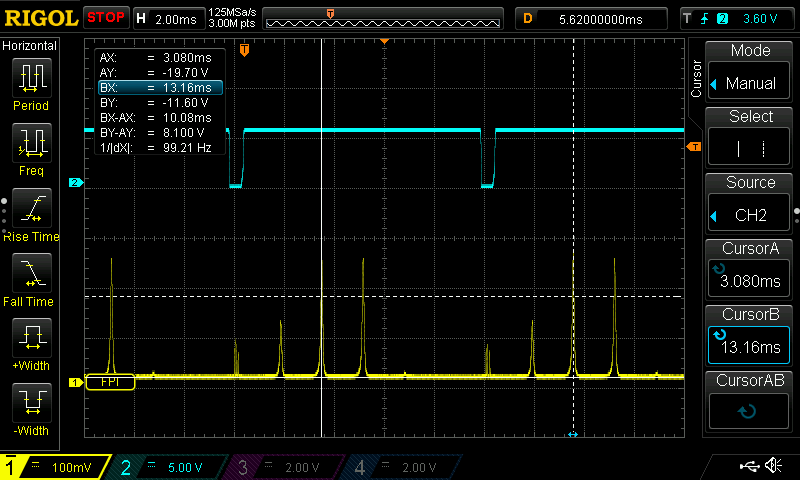
\includegraphics[width = \linewidth]{Bilder/Auswertung/FabryPerotKalibr.png}
    \caption{Longitudinale Lasermoden mit dem Fabry-Pérot aufgenommen. Channel 1 ist das Messsignal und Channel 2 ist des Triggersignal des Interfermoters. Gekennzeichnet sind 
    mit den x-Marker zwei gleich Peaks.}
    \label{bild:FreierSpektralbereich}
\end{figure}


\subsection*{Abstand und Linienbreite Axialer Lasermoden}

Den Abstand der Moden bestimmt man auch grafisch aus Abbildung \ref{bild:AxialModenAbstand}. Aus diesem erhält man 
\begin{equation*}
    \Delta t = (1,660 \pm 0,086)\,\mathrm{ms}
\end{equation*}
und mit der Umrechnung aus Gleichung \ref{eq:Umrechnung} erhalt man 

\begin{equation}
    \textcolor{red}{\delta \nu = (252 \pm 17)\,\mathrm{MHz}}
    \label{eq:Modenabstand}
\end{equation}

den Abstand zweier longitudinaler Lasermoden. Die Unsicherheit wird hierbei aus geschätzter Ableseunsicherheit und
der Unsicherheit der Kalibrierung mittels Fehlerfortpflanzung berechnet. Auf selbe Weise wird 

\begin{equation}
    \textcolor{red}{\Delta \nu_{multi} = (13,3 \pm 1,5)\,\mathrm{MHz}}
\end{equation}

auch die Linienbreite (FWHM) aus Abbildung \ref{bild:Lininebreite} bestimmt. Gleiches tun wir auch für die einzelne Mode
aus Abbildung \ref{bild:LininebreiteSingle}. Damit erhalten wir die Werte, welche in Tabelle \ref{tab:Linienbreite} dargestellt sind.

\begin{table}
    \centering
 
    \begin{tabular}{lcr}
        \toprule
        Messgröße & Symbol & Wert in MHz\\
        \midrule
        Freier spektraler Bereich& $\Delta \nu_{FSB}$ & 2000\\
        Modenabstand& $\delta\nu$& $252 \pm 17$\\
        FWHM (multi-mode)& $\Delta\nu_{multi}$&$13,3 \pm 1,5$\\
        FWHM (single)& $\Delta\nu_{single}$&$16,7 \pm 2,6$\\
        \bottomrule        
    \end{tabular}
  
    \caption{Freier spektraler Bereich, Modenabstand, Halbwertsbreite des He-Ne-Laser und dem dazugehörendem 
    konfokalem Fabry-Pérot-Interferometer}
    \label{tab:Linienbreite}
\end{table}


\subsection*{Verstärkungsprofil}

Um das Verstärkungsprofil zu bestimmen haben wir das Oszilloskop auf einen Modus gestellt, bei dem es alle Spuren 
überlagert. Dies haben wir getan und haben den Tisch mit leichten Erschütterungen zum Vibrieren gebracht.
Dies führte zu dem benötigten Längenänderungen im Resonator, sodass die Peaks der Moden gewackelt haben.
Somit kann man, wenn man mit den Linien wackelt, ein ungefähres Bild bekommen, wie das Verstärkungsprofil
des Verstärkers aussieht. Das Ergebnis ist in Abbildung \ref{bild:Verstaerkung} sichtbar.

\begin{figure}[h]
    \centering
    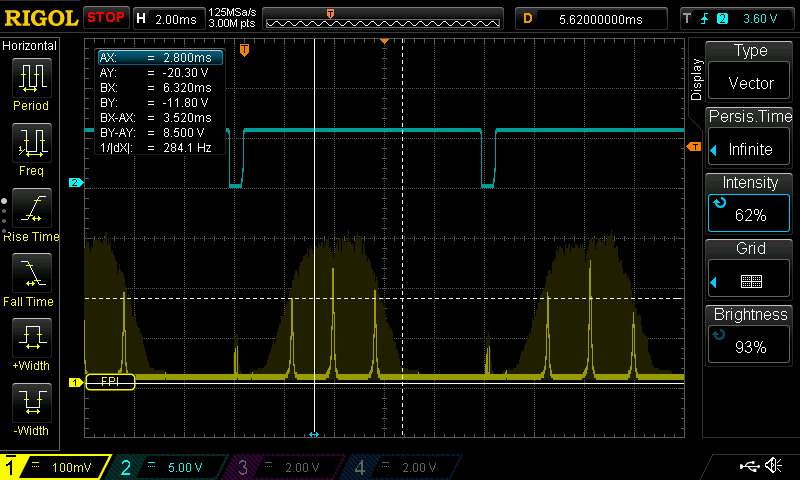
\includegraphics[width = \linewidth]{Bilder/Auswertung/FabryPerotVerst.png}
    \caption{Longitudinale Lasermoden mit dem Fabry-Pérot aufgenommen. Durch Erschütterung wurde das Verstärkungsprofil sichtbar gemacht.}
    \label{bild:Verstaerkung}
\end{figure}

Von diesem schätzen wir die Halbwertsbreite ab, soweit möglich. Die Halbwertsbreite 

\begin{equation}
    \textcolor{red}{\Delta\nu_{Verstaerkungsprofil} = 532 \pm 80 \, \mathrm{MHz}}
\end{equation}

hat einen relativ großen Fehler, da man die Spitze des Verstärkungsprofils nicht genau sehen kann und daher abschätzen muss.
Dies ist auch sinnvoll, da die Breite des Verstärkungsprofils mehrmals den Modenabstand beinhalten sollte.


\subsection*{Finesse und Auflösungsvermögen}

Die Finesse und das Auflösungsvermögen sind zwei Größen, die zur Charakterisierung des Resonators nützlich sind. Die Finesse ist dabei
definiert über das Verhältnis 
\begin{align}
    \mathcal{F} = \frac{\delta \nu_{FSR}}{\Delta\nu} \qquad s_{\mathcal{F}} = \sqrt{(\frac{s_{\Delta \nu}*\delta \nu_{FSR}}{\Delta\nu^2})^2+(\frac{s_{\delta\nu}}{\Delta \nu})^2}
\end{align}
 des freien Spektralbereichs zur Linienbreite. Die Auflösung 

 \begin{align}
     A = \frac{\nu}{\Delta\nu} = \frac{c}{\lambda\Delta\nu} \qquad s_A = A\sqrt{(\frac{s_{\Delta\nu}}{\Delta\nu})^2} = A\frac{s_{\Delta\nu}}{\Delta\nu}
 \end{align}
 
 ist hingegen das Verhältnis der Linienbreite zur Frequenz der Spektrallinie. Dabei wurde die Frequenz durch
 die Lichtgeschwindigkeit $c$ und die angegeben Wellenlänge $\lambda$ des Lasers (632,8\,nm) berechnet. 
 
 \begin{gather}
    \textcolor{red}{\mathcal{F} = 119\pm19}\\
    \textcolor{red}{A = (28,3\pm4,4)\cdot10^6}
 \end{gather}


 \subsection*{Mischfrequenzen}

 Mit Hilfe einer Photodiode wollen wir versuchen die Mischfrequenz der Moden zu bestimmen. Dies tun wir, um den Frequenzabstand zu verifizieren. 
 Dabei können wir leider nicht das elektrische Feld anhand seiner Intensität direkt messen, da dieses zu hochfrequent ist. Was wir aber messen können, sind 
 die niederfrequenten Anteile, welche sich aus den Mischtermen ergeben. Dabei erwarten wir in etwa den Modenabstand zu erhalten. 
 Bei der Aufnahme ist es relativ schwierig einen Wert abzulesen, da wir zwei kleine Peaks nebeneinander sehen. Die Mischfrequenz 
 \begin{equation*}
     \textcolor{red}{\Delta \nu_{Misch1} = (281,93\pm0,40)\,\mathrm{MHz} }
 \end{equation*}

 hat trotzdem noch deutlich weniger Unsicherheit als der vorher bestimmte Wert. Dabei ist der Wert nahe an dem Wert des 
 Modenabstandes aus Tabelle \ref{tab:Linienbreite}, aber nicht ganz. Die Messunsicherheiten der beiden Messungen überlappen leider nicht. Das ist ein Hinweis darauf, dass es noch Fehlerquellen im Hintergrund gibt, welche wir nicht
 berücksichtigt haben.

 \subsection*{Laser als Längenmessgerät}

 Durch das Einbringen eines Glasplättchen verlängern wir den optischen Weg im Resonator. Dabei müssen wir 
 festhalten, dass es sich bei unserem Resonator um einen konfokalen Resonator handelt. Es sieht im Spektrum so aus, 
 als hätten wir den Resonator verlängert. Diese Verlängerung 

 \begin{equation*}
     \Delta L = d*n - d
 \end{equation*}

 berechnet sich aus der Dicke $d$ des Plättchens und dem Brechungsindex $n$ des Glasplättchens. Allgemein ist der 
 Modenabstand 
 
 \begin{equation*}
     \Delta\nu = \frac{c}{2L\cdot n}
 \end{equation*}

 abhängig von der Länge des Resonators. Bei einem konfokalem Laser ist er sogar abhängig von 

 \begin{equation*}
    \Delta\nu = \frac{c}{4L\cdot n},
\end{equation*}

da der Laserstrahl vier Mal L zurücklegen muss um mit sich selbst zu interagieren\footnote{\url{https://www.uni-muenster.de/Physik.AP/Denz/Studieren/Lehrveranstaltungen/photonik_ws1213_laser.html}, Eingesehen: 07.10.2021}
Damit ergibt sich bei für die Dicke 

\begin{equation}
    d = \frac{c}{4(n-1)}\cdot \biggl( \frac{1}{\Delta\nu_{Misch2}}-\frac{1}{\Delta\nu_{Misch2}} \biggl)
\end{equation}


des Plättchens, wobei Mischfrequenz 2 $\Delta \nu_{Misch2} = (281,90\pm0,40)\,\mathrm{MHz}$ die Frequenz des verlängerten Resonators ist. \\
Mit dem Brechungsindex von 1,54 \cite[S.1358]{Chemie1949} erhält man 

\begin{equation}
    \textcolor{red}{d = (0,05 \pm 0,90)\,\mathrm{mm,}}
\end{equation}

was aber ein unrealistischer Wert ist. Man sieht daran, dass es sich die Methode mäßig zum bestimmen von Längen eignet. Das liegt unter anderem daran, dass die
Abstände der Mischfrequenzen viel kleiner als ihre Fehler sind. Bei größeren Unterschieden sollte die Methode jedoch funktionieren. 